% VUT FIT MITAI
% MSZ 2021/2022
% Author: Vladimir Dusek
% Login: xdusek27

%%%%%%%%%%%%%%%%%%%%%%%%%%%%%%%%%%%%%%%%%%%%%%%%%%%%%%%%%%%%%%%%%%%%%%%%%%%%%%%%

% Path to figures
\graphicspath{{pds/smerovace/figures}}

%%%%%%%%%%%%%%%%%%%%%%%%%%%%%%%%%%%%%%%%%%%%%%%%%%%%%%%%%%%%%%%%%%%%%%%%%%%%%%%%

\chapter{PDS -- Základní funkce směrovače, zpracování paketů ve směrovači, typy přepínání a architektur.}

%%%%%%%%%%%%%%%%%%%%%%%%%%%%%%%%%%%%%%%%%%%%%%%%%%%%%%%%%%%%%%%%%%%%%%%%%%%%%%%%

\section{Metadata}

\begin{compactitem}
    \item Předmět: Přenos dat, počítačové sítě a protokoly (PDS)
    \item Přednáška:
    \begin{compactitem}
        \item \path{05-routing.pdf}
    \end{compactitem}
    \item Záznam:
    \begin{compactitem}
        \item 2021-03-12
    \end{compactitem}
\end{compactitem}

%%%%%%%%%%%%%%%%%%%%%%%%%%%%%%%%%%%%%%%%%%%%%%%%%%%%%%%%%%%%%%%%%%%%%%%%%%%%%%%%

\section{Úvod a kontext}

\textit{Viz. \uv{Úvod a kontext} v~předchozích otázkách z~tohoto předmětu.}

\paragraph*{NAT} NAT (\textit{Network Address Translation}) je metoda mapování IP adresního prostoru do jiného prostoru (typicky privátní adresy na veřejné adresy). Děje se tak úpravou hlaviček IP paketů během jejich přenosu přes směrovače.

\paragraph*{ACL} ACL (\textit{Access Control List}) je volitelná vrstva zabezpečení, která funguje jako brána firewall pro řízení provozu do jedné nebo více podsítí a z nich.

\paragraph*{ARP} ARP (\textit{Address Resolution Protocol}) a RARP (\textit{Reverse ARP}) je protokol, který komunikuje na síťové vrstvě (L3) a zajišťuje \uv{překlad} IP adres na MAC adresy a obráceně. Pouze pro IPv4, pro IPv6 je pro stejný účel využíván protokol ICMPv6 a zpráva \textit{Neighbor Discovery}.

\paragraph*{ICMP} ICMP (\textit{Internet Control Message Protocol}) je protokol, který komunikuje na síťové vrstvě (L3) a slouží pro řízení toku a detekce nedosažitelných uzlů.

\paragraph*{MTU} MTU (\textit{Maximum Transmission Unit}) je největší velikost paketu, kterou lze v síti odeslat (přes výstupní rozhraní síťového prvku). Závisí na síťové kartě příslušného rozhraní.

\paragraph*{Fragmentace paketů} Uzel v síti (směrovač) dostane paket o velikosti $n$. Paket má přeposlat přes výstupní rozhraní do sítě, ve které je $MTU < n$. Aby paket mohl být odeslán, musí být rozdělen (fragmentován) na více menších paketů (fragmenty) a odeslán po částech. Na straně příjemce pak musí nastat opačný proces~--~defragmentace.

%%%%%%%%%%%%%%%%%%%%%%%%%%%%%%%%%%%%%%%%%%%%%%%%%%%%%%%%%%%%%%%%%%%%%%%%%%%%%%%%

\section{Základní popis směrovače}

Směrovač je síťové zařízení, které předává datové pakety mezi počítačovými sítěmi. Základní charakteristika: \begin{compactitem}
    \item Směrovač pracuje s pakety (síťová vrstva, L3).
    \item Tvoří rozhraní mezi počítačovými sítěmi (provádí překlad NAT).
    \item Klasifikuje a filtruje pakety (firewall).
    \item Provádí fragmentaci a defragmentaci.
\end{compactitem}

% \todo{todo} ACL

\paragraph*{Činnost} \begin{compactenum}
    \item Vypouzdření paketu z L2 (odebrání L2 hravičky) a kontrola jestli je v pořádku (pomocí kontrolního součtu).
    \item Vyhledání cesty kam se má paket směrovat a překlad adresy NAT (pomocí směrovací tabulky).
    \item Určení cílové MAC adresy na základě cílové IP adresy (pošle ARP dotaz).
    \item Určení výstupního rozhraní.
    \item Sestavení výsledného paketu podle výstupního rozhraní (zapouzdření do příslušné L2 technologie -- přidání L2 hlavičky).
\end{compactenum}

\paragraph*{Co ovlivňuje propustnost} \begin{compactitem}
    \item Rozbalení paketu.
    \item Vyhledání směrovací cesty.
    \item Překlad NAT.
    \item Vyhledání cílové MAC adresy.
    \item Zabalení paketu do správné technologie.
\end{compactitem}

\paragraph*{Typy} \begin{compactitem}
    \item Páteřní směrovače -- součástí pátečních sítí mezi ISP.
    \item Hraniční směrovače -- mezi zákaznickými sítěmi a ISP.
    \item Podnikové směrovače -- propojení koncových systému v podnikových (\textit{enterprise}) sítích.
    \item Domácí směrovače.
\end{compactitem}

%%%%%%%%%%%%%%%%%%%%%%%%%%%%%%%%%%%%%%%%%%%%%%%%%%%%%%%%%%%%%%%%%%%%%%%%%%%%%%%%

\section{Operace co směrovač vykonává}

Pakety mohou být určeny buď přímo pro směrovač (aktualizace směrovací cesty přes směrovací protokoly -- aktualizace směrovací tabulky) a nebo jinému uzlu v síti. V takovém případě směrovač paket přeposílá dalším uzlům v síti.

\begin{compactitem}
    % \item Základní operace směrovače jsou definovány v RFC a musí je implementovat každý směrovač.
    \item \textbf{Směrování} (\textit{routing}) -- Určování cest paketů v prostředí počítačových sítí. Směrování zajišťují nejen routery, ale i koncové stanice (při vysílání) a jeho úkolem je doručit paket adresátovi, pokud možno co nejefektivnější cestou.
    \item \textbf{Přepínání} (\textit{forwarding, switching}) -- Přepnutí paketu ze vstupního rozhraní na výstupní (viz architektura přepínačů).
\end{compactitem}

\begin{figure}[H]
    \centering
    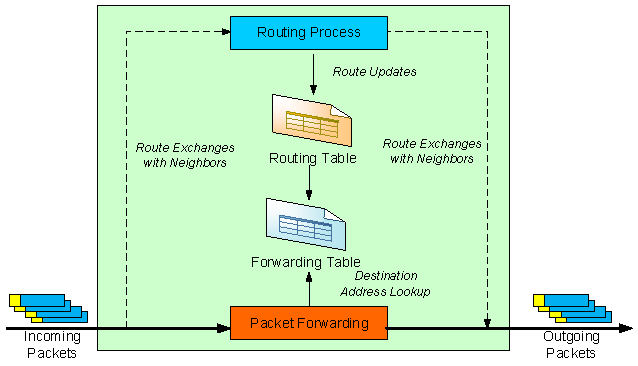
\includegraphics[width=1\linewidth]{smerovac_nakres.pdf}
    \caption{Základní činnost směrovače.}
\end{figure}

\paragraph*{Směrovací tabulka} Směrovací tabulka (\textit{routing table}) obsahuje informace nutné a dostačující pro směrování (\path{ip prefix} -- prefix cílové sítě, \path{next hop} -- adresa dalšího uzlu, \path{metrika} -- cena cesty). Informace do ní se získavají pomocí směrovacích protokolů a nebo staticky (administrátor provede manuálně).

\begin{figure}[H]
    \centering
    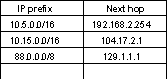
\includegraphics[width=0.4\linewidth]{smerovaci_tabulka.pdf}
    \caption{Příklad směrovací tabulky (bez metriky).}
\end{figure}

\paragraph*{Přepínací tabulka} Přepínací tabulka (\textit{forwarding table}) doplňuje směrovací tabulku o další informace, které jsou nutné pro sestavení cílového paketu (výstupní rozhraní, zdrojová MAC adresa, cílová MAC adresa). Informace do ní se získavají pomocí ARP protokolu a doplnění vlastních informací (\texttt{dst MAC address}).

\begin{figure}[H]
    \centering
    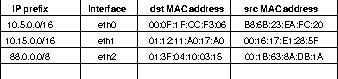
\includegraphics[width=0.9\linewidth]{prepinaci_tabulka.pdf}
    \caption{Příklad přepínací tabulky.}
\end{figure}

\begin{figure}[H]
    \centering
    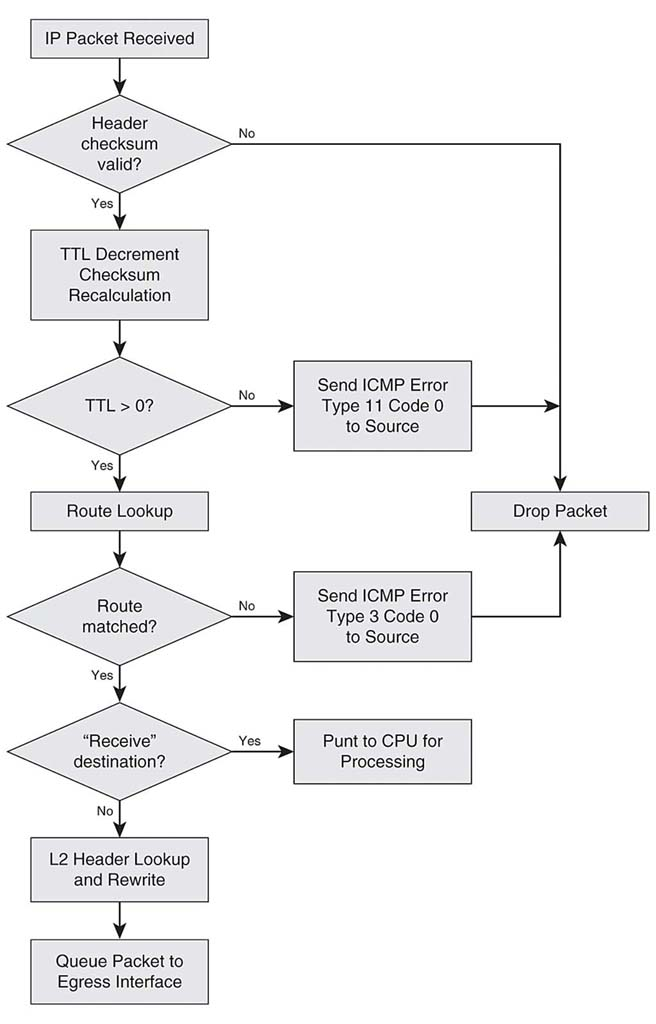
\includegraphics[width=0.75\linewidth]{cinnost_smerovace.png}
    \caption{Diagram zpracování paketu ve směrovači.}
\end{figure}

\paragraph*{Základní operace podrobněji} \begin{compactenum}
    \item Validace hlavičky L3 (formát, verze, délka).
    \item Kontrola hodnoty TTL a její dekrementace. Pokud je TLL 0, tak se paket zahodí a pošle ICMP zpráva.
    \item Přepočítání kontrolního součtu.
    \item Zpracování rozšířených voleb IP protokolu (timestamp, record route, strict source route).
    \item Vyhledání cesty (next-hop) na základě cílové adresy (lokální doručení, unicast, multicast). Pokud se nepodaří vyhledat cesta, tak se paket zahodí a pošle ICMP zpráva.
    \item Fragmentace a defragmentace IP paketů (pokud $MTU_{in} < MTU_{out}$).
    \item Zpracování zpráv ICMP a IGMP.
\end{compactenum}

%%%%%%%%%%%%%%%%%%%%%%%%%%%%%%%%%%%%%%%%%%%%%%%%%%%%%%%%%%%%%%%%%%%%%%%%%%%%%%%%

\section{Architektura směrovače}

Rozdělíme na fyzické části (z hlediska hardware) a funkční části (z hlediska komponent co něco vykonávají).

\subsection{Fyzické části}

\begin{compactitem}
    \item Procesorová část (\textit{Router Processor Card})
    \item Přepínací logika (\textit{Switch Fabric Card})
    \item Síťové karty (\textit{Line Card}) -- každá má vstupní a výstupní rozhraní (\textit{Port Card})
\end{compactitem}

\begin{figure}[H]
    \centering
    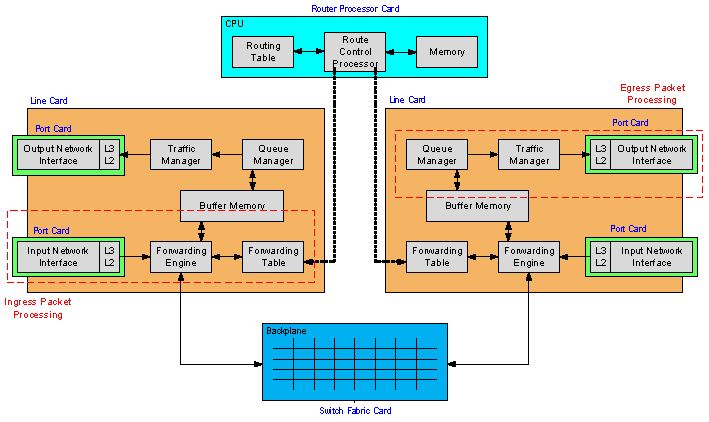
\includegraphics[width=1\linewidth]{architektura_fyzicke_casti.pdf}
    \caption{Fyzické části (procesory, paměti) směrovače.}
\end{figure}

\subsection{Funkční části}

\paragraph*{Procesorová část} procesor, paměť, směrovací tabulka \begin{compactitem}
    \item Implementuje směrování na obecném CPU
    \item Zpracovává směrovací informace: aktualizace, udržuje sousedství
    \item Obsluhuje směrovací tabulku
    \item Přenáší data do přepínací tabulky
    \item Zpracovává pakety, které nelze směrovat pomocí FIB
    \item Vytváří chybové zprávy ICMP
\end{compactitem}

\paragraph*{Přepínací logika} propojovací deska (\textit{Backplane})\begin{compactitem}
    \item Propojuje síťové rozhraní
    \item Vytváří sdílené (shared) či přepínané (switched) propojení
    \item Rychlost přepínání odpovídá přenosovému pásmu všech rozhraní
\end{compactitem}

\paragraph*{Síťové karty} \begin{compactitem}
    \item Vstupní/Výstupní síťové rozhraní (\textit{Input/Output Network Interface}) \begin{compactitem}
        \item Obsahuje více vstupních/výstupních portů
        \item Odstraní zapouzdření L2
        \item Předá hlavičku L3 přepínacímu modulu
        \item Uloží paket do paměti
        \item Zapouzdří odchozí pakety
    \end{compactitem}
    \item Řízení přepínání (\textit{Forwarding Engine}) \begin{compactitem}
        \item Dostane hlavičku L3 ze síťového rozhraní
        \item Určí výstupní rozhraní podle informace ve FIB
        \item Provádí klasifikace paketů pro podporu QoS na výstupu
    \end{compactitem}
    \item Správce front (\textit{Queue Manager}) \begin{compactitem}
        \item Ukládá pakety do vyrovnávací paměti, pokud je výstupní port obsazen
        \item Spravuje výstupní frontu $\rightarrow$ různé typy výstupních front
        \item Při zaplnění fronty vybírá a zahazuje pakety podle definované politiky
    \end{compactitem}
    \item Správce provozu (\textit{Traffic Manager}) \begin{compactitem}
        \item Prioritizuje a reguluje výstupní provoz podle požadavků QoS
        \item Omezuje či ořezává výstupní provoz (shaping, policing)
    \end{compactitem}
\end{compactitem}

\begin{figure}[H]
    \centering
    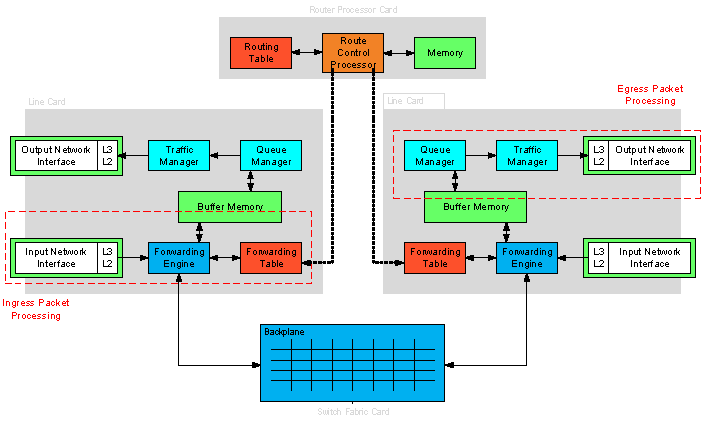
\includegraphics[width=1\linewidth]{architektura_funkci_casti.pdf}
    \caption{Funkční částí (procesy).}
\end{figure}

%%%%%%%%%%%%%%%%%%%%%%%%%%%%%%%%%%%%%%%%%%%%%%%%%%%%%%%%%%%%%%%%%%%%%%%%%%%%%%%%

\section{Zpracování paketu ve směrovači}

Data Plane -- specifický hardware pro zpracování

Control Plane -- obecný procesor se softwarem, který běží (NAT, filtrovani pomoci ACL/firewall, fragmenta, defragmentace se obvykle musí zpracovávat tady)

kontext paketu -- vybrané věci z hlaviček, který se předává, datová struktura, nepracuju s celým paketem
na začátku mám pouze částečný kontext (síťová karta), na výstupní kartě mám už kompletní

pricina zahozeni na vystupni karte -- TTL, plne fronty (politiky RED, WRED), filtrovani na vstupu/vystupu

Rychlá cesta (pouze hw)
casove kriticke operace
zpracování hlavičky IP
klasifikace

Pomalá cesta (vlastní řízení, přes obecný software)
částěčně zpracována v HW, částečně v softwaru (control plane)
časově nekritické operace
zpracování ARP

%%%%%%%%%%%%%%%%%%%%%%%%%%%%%%%%%%%%%%%%%%%%%%%%%%%%%%%%%%%%%%%%%%%%%%%%%%%%%%%%

\section{Typy přepínání}

Softwarové přepínání (\textit{Process Switching})

Rychlé přepínání (\textit{Fast Switching})

%%%%%%%%%%%%%%%%%%%%%%%%%%%%%%%%%%%%%%%%%%%%%%%%%%%%%%%%%%%%%%%%%%%%%%%%%%%%%%%%

\section{Přehled architektur}

Architektura se sdíleným procesorem

Architektura s nezávislými moduly FE

Distribuovaná architektura (Shared Nothing)
